% =============================================================================
% File:  sample_slides.tex --  Example of the use of the Falkor Beamer theme
% Author(s): Sebastien Varrette <Sebastien.Varrette@uni.lu>
% Time-stamp: <Lun 2013-12-02 22:23 svarrette>
% 
% Copyright (c) 2012 Sebastien Varrette <Sebastien.Varrette@uni.lu>
% .             http://varrette.gforge.uni.lu
% 
% For more information:
% - LaTeX: http://www.latex-project.org/
% - Beamer: https://bitbucket.org/rivanvx/beamer/
% - LaTeX symbol list:
% http://www.ctan.org/tex-archive/info/symbols/comprehensive/symbols-a4.pdf
% 
% Latest version of these files can be found on Github:
% 

% =============================================================================
\documentclass{beamer}
% \documentclass[draft]{beamer}
\usepackage{_style}

% The key part to use my theme
\usetheme{Falkor}

% Not integrated in my theme as not everybody wants that
\AtBeginSection[]
{
  \frame{
    \frametitle{Summary}
    {\scriptsize\tableofcontents[currentsection]}
  }
}

%%%%%%%%%%%%%%%%%%%%%%%%%%%% Header %%%%%%%%%%%%%%%%%%%%%%%%%%%%%%
\title{The \texttt{Falkor} \LaTeX Beamer Style}
\subtitle{Overview and Usage}

\author{S\'ebastien Varrette}
\institute[CSC research unit]{
  Computer Science and Communications (CSC) Research Unit,
  University of Luxembourg, Luxembourg
}

% Mandatory to define a logo - otherwise compilation will fail in an unobvious
% manner.
\pgfdeclareimage[height=0.8cm]{logo}{Images/logo_UL.pdf}
\logo{\pgfuseimage{logo}}
\date{}

%%%%%%%%%%%%%%%%%%%%%%%%%%%%%% Body %%%%%%%%%%%%%%%%%%%%%%%%%%%%%%%
\begin{document}

\begin{frame}
    \vspace{2.5em}
    \titlepage
\end{frame}

% .......
\frame{
  \begin{center}
      \textbf{Latest versions available on
        \href{https://github.com/Falkor/}{Github}}:
      \vfill
      \begin{description}
        \item[Beamer theme Falkor:] \hfill
          \myurl{https://github.com/Falkor/beamerthemeFalkor}
        \item[Generic Makefiles:] \hfill
          \myurl{https://github.com/Falkor/Makefiles}
        \item[Git bootstrapping script:] \hfill
          \myurl{https://github.com/Falkor/Makefiles/blob/devel/scripts/}
      \end{description}
  \end{center}
}

% ......
\frame{
  \frametitle{Summary}
  {\scriptsize
    \tableofcontents
  }
}

% ===============================================
\section{Installation}

% ........................
\frame[containsverbatim]{
  \frametitle{Basic usage}

  \begin{block}{}%Bootstrap a new working directory}
      \begin{itemize}
        \item Get the latest version on
          \href{https://github.com/Falkor/beamerthemeFalkor}{Github}
          \begin{cmdline}
              \cmdlineentry{cd /path/to/cloning/dir}\\
              \cmdlineentry{git clone https://github.com/Falkor/beamerthemeFalkor.git}
          \end{cmdline}

        \item Copy \href{https://github.com/Falkor/beamerthemeFalkor/blob/master/beamerthemeFalkor.sty}{beamerthemeFalkor.sty} at the root of your \LaTeX document


        \item Place the following code on your \LaTeX\ file:
          \begin{lstlisting}[basicstyle=\tiny,numbers=none]
              \usetheme{Falkor}
          \end{lstlisting}

        \item That's all (normally).
          \begin{itemize}
              \itemhook you might want to use my \href{https://github.com/Falkor/Makefiles/blob/devel/latex/Makefile}{Generic Makefile for \LaTeX}
          \end{itemize}

          % \item Duplicate the sample structure of the freshly cloned repository
          %   \begin{cmdline}
          %       \cmdlineentry{cd /path/to/working/dir}\\
          %       \cmdlineentry{rsync -avzu --exclude "*.git" $\backslash$\\ ~~~~~/path/to/cloning/dir/beamerthemeFalkor/ .}
          %   \end{cmdline}
          % \item Copy and adapt the sample document \texttt{sample\_slides.tex}
          %   \begin{itemize}
          %     \item[$\hookrightarrow$] run \texttt{make} to generate \texttt{sample\_slides.pdf}
          %   \end{itemize}
      \end{itemize}
  \end{block}
}

% .......
\frame{
  \frametitle{Full sample example \hfill{\tiny (\textit{i.e.} these slides)}}

  \begin{block}{}
      \begin{itemize}
        \item To copy a full working example
          \begin{cmdline}
              \cmdlineentry{cd /path/to/cloning/dir}\\
              \cmdlineentry{git clone https://github.com/Falkor/beamerthemeFalkor.git}\\
              \cmdlineentry{cd /path/to/working/dir}\\
              \cmdlineentry{rsync -avzu -L --exclude "*.git" $\backslash$\\~~~~~~~/path/to/cloning/dir/beamerthemeFalkor/ .}\\
              \cmdlineentry{make}
          \end{cmdline}
      \end{itemize}
  \end{block}
  \begin{itemize}
    \item This will generate the file \texttt{sample\_slides.pdf}.
      \begin{itemize}
          \itemhook adapt accordingly...
      \end{itemize}
  \end{itemize}

}




\frame{
  \frametitle{The scripted appraoch}

  \begin{block}{Git sub-modules approach}
      \begin{itemize}
        \item Assuming you want to use the theme in an existing git repo
          \begin{cmdline}
              \cmdlineentry{cd /path/to/working/dir}\\
              \cmdlineentry{git submodule add $\backslash$\\
                ~~~~~https://github.com/Falkor/beamerthemeFalkor.git
                $\backslash$\\
                ~~~~~.beamerthemeFalkor}\\
              \cmdlineentry{ln -s
                .beamerthemeFalkor/beamerthemeFalkor.sty .}
          \end{cmdline}
      \end{itemize}
  \end{block}
}

\frame{
  \frametitle{Changing the logo}

  \begin{itemize}
    \item The logo used by the theme is \texttt{images/slide\_image.jpg}
    \item To use another logo:
      \begin{cmdline}
          \cmdlineentry{cd images}\\
          \cmdlineentry{wget http://path/to/myimage.jpg}\\
          \cmdlineentry{ln -sf myimage.jpg slide\_image.jpg}\\
      \end{cmdline}
  \end{itemize}
}

% ===============================================
\section{Some example slides}

% ............
\frame{

  \frametitle{Objectives of our work}

  \begin{itemize}
    \item Better than assumptions/\textit{a-priori}: concrete models and
      experiments
  \end{itemize}

  \begin{alertblock}{}
      \begin{itemize}
        \item Evaluate impact of the underlying hypervisor
          \begin{itemize}
              \itemhook at the heart of \textbf{any} cloud middleware so far
              % \itemhook analysis of the most widespread virtualization
              % frameworks
              \itemhook \emph{lightweight},
              \emph{high-level} model of a \emph{virtualized} machine.
          \end{itemize}
        \item Evaluate a real HPC platform (or anything as close as possible)
          \begin{itemize}
              \itemhook concrete deployment on top of the Grid5000 platform
              \itemhook select benchmarking tools to reflect an HPC usage
          \end{itemize}
      \end{itemize}
  \end{alertblock}


  ~\vfill
  {\tiny
    \mycite{SBAC-PAD13} S. Varrette,  M. Guzek, V. Plugaru, J. E. Sanchez, and P. Bouvry.
    "\textit{HPC Performance and Energy-Efficiency of Xen, KVM and VMware Hypervisors}". In Proc. of the 25th IEEE Symposium on Computer Architecture and High Performance (SBAC-PAD'13), Oct 2013.
    % Do not forget the below space

  }

}


% .......
\frame[t]{
  \frametitle{The Grid'5000 Testbed \hfill \myurl{http://www.grid5000.fr}}

  \begin{itemize}
    \item Large scale nation wide infrastructure \hfill
\includegraphics{logo_G5K.png}
      \begin{itemize}
          \itemhook for large scale parallel and distributed computing research.
      \end{itemize}

  \end{itemize}
  % ~~~~~~~~~~~~~~
  \begin{columns}
      \column{0.4\textwidth}
      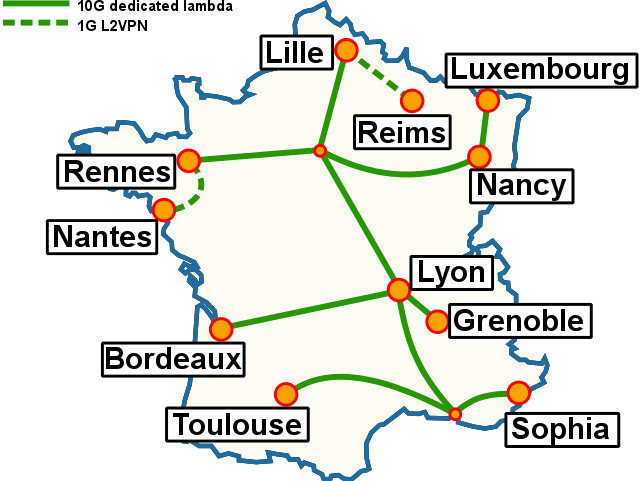
\includegraphics[scale=0.9]{Renater5-g5k.jpg}
      \column{0.6\textwidth}
      \begin{itemize}
        \item 10 sites in France
        \item \emph{Abroad}: Luxembourg, Porto Allegre
        \item Total: \textbf{7896} cores over \textbf{26} clusters
        \item 1-10GbE / Myrinet / Infiniband interconnect
        \item \emph{Kadeploy} functionnality
      \end{itemize}
  \end{columns}
}


\frame[containsverbatim]{
  \frametitle{A slide with listings}%\frametitle{Problem}
  \begin{block}{A JavaScript program}
      \begin{lstlisting}[basicstyle=\tiny,numbers=none]
          function fibo(n)
          {
            if( n <= 1 )
            {
              return n;
            }
            var res = fibo(n-1) + fibo(n-2);
            return res;
          }
          n = parseFloat(arguments[1])
          nn = fibo(n)
          print(nn)
      \end{lstlisting}

  \end{block}

}


\section{Conclusion}

% ............
\begin{frame}
    \frametitle{Conclusion}

    \begin{itemize}
      \item Summary point 1
      \item Summary point 2
    \end{itemize}

    \begin{block}{Perspectives}
        \begin{itemize}
          \item Improve point 1
          \item Improve point 2
        \end{itemize}
    \end{block}


\end{frame}


% ======================== END =========================

\section*{Thank you for your attention...}
\frame{
  \frametitle{Questions?}
  \begin{center}
      
\includegraphics[scale=0.2]{question.jpg}
  \end{center}

  {\tiny
    \tableofcontents

  }
}

\newcounter{finalframe}
\setcounter{finalframe}{\value{framenumber}}

% \appendix

\frame{
  \frametitle{Appendix}

  \begin{acronym}\setlength\itemsep{-0.3em}
      \acro{DFT}{Discrete Fourier Transform}
      \acro{EA}{Evolutionary Algorithm}
      \acro{PRNG}{[Pseudo]-Random Number Generator}
      \acro{UL}{University of Luxembourg}
  \end{acronym}

  \textit{*Note: notice the slide number below...}
}

% .......
\frame{
  \frametitle{Another appendix slide}

  \textit{Note again the slide number below...}

}


\setcounter{framenumber}{\value{finalframe}}

\end{document}

% ~~~~~~~~~~~~~~~~~~~~~~~~~~~~~~~~~~~~~~~~~~~~~~~~~~~~~~~~~~~~~~~~
% eof
% 
% Local Variables:
% mode: latex
% mode: flyspell
% mode: auto-fill
% fill-column: 80
% End:
